\section{Results}

We evaluate delta-based tile scoring (DTS) against MInference, FlexPrefill, and XAttention. We exclude SpargeAttention from our comparisons because its implementation is bundled with quantization. All baselines are run directly from their original GitHub repositories without reimplementation. We report DTS at two cosine thresholds, 0.72 and 0.78. Across all applicable methods, we use a recall or coverage target of 0.90 (i.e., $r{=}0.90$ for DTS and XAttention, and $\gamma{=}0.90$ for FlexPrefill). We evaluate these methods on RULER and LongBench, alongside an isolated speedup analysis from 4K to 512K tokens.


\subsection{RULER}

Table~\ref{tab:delta_tile_scoring} reports RULER accuracy. DTS achieves near-lossless performance, with both threshold settings outperforming every sparse baseline tested. The performance gap is most pronounced at 128K tokens: DTS maintains scores of 75.55 (cos\,0.78) and 74.82 (cos\,0.72), whereas XAttention drops to 70.96 ($s{=}16$) and 71.57 ($s{=}8$), and MInference falls more severely to 63.73.

\begin{table}[!ht]
\centering
\caption{RULER accuracy (\%) comparing delta-based tile scoring against baseline and block-sparse methods on LLaMA-3.1 8B Instruct. Best score per column in \textbf{bold}.}
\label{tab:delta_tile_scoring}
\resizebox{\linewidth}{!}{%
\begin{tabular}{lrrrrrrr}
\toprule
Method & 4K & 8K & 16K & 32K & 64K & 128K & Avg \\
\midrule
Full attention              & 96.16 & 93.77 & 93.43 & 90.47 & \textbf{86.14} & 74.46 & \textbf{89.07} \\
MInference                  & 96.04 & 93.95 & 92.60 & 88.43 & 84.66 & 63.73 & 86.57 \\
FlexPrefill                  & 95.37 & 92.29 & 91.23 & 88.02 & 83.56 & 74.23 & 87.45 \\
\midrule
XAttn $s{=}16$                & \textbf{96.17} & 93.97 & 93.43 & 90.56 & 83.04 & 70.96 & 88.02 \\
XAttn $s{=}8$                 & 95.57 & 93.92 & 92.71 & \textbf{90.60} & 81.83 & 71.57 & 87.70 \\
\midrule
DTS cos\,0.72 & 95.83 & \textbf{94.22} & 93.36 & 90.42 & 85.19 & 74.82 & 88.97 \\
DTS cos\,0.78 & 96.14 & 93.70 & \textbf{93.44} & 90.35 & 84.93 & \textbf{75.55} & 89.02 \\
\bottomrule
\end{tabular}%
}
\end{table}

\subsection{LongBench}
\label{sec:results_longbench}

Table~\ref{tab:longbench} shows that DTS is the strongest sparse method on average, nearly matching full attention. However, performance varies by task. On multi-hop reasoning (2WikiMultiHopQA) and LCC, cos\,0.72 matches or exceeds the baseline while cos\,0.78 slightly trails. Summarization is robust across all methods, while DTS excels on passage retrieval and RepoBench-P, exactly matching or significantly beating full attention. While DTS slightly trails baselines on TREC for LLaMA, it achieves the highest score on Qwen, indicating this is not a systematic flaw.


\begin{table*}[!ht]
\centering
\small
\caption{LongBench scores on LLaMA-3.1 8B Instruct. NQA = NarrativeQA, Qas = Qasper, MFQ = MultifieldQA-en, HotP = HotpotQA, 2Wiki = 2WikiMultiHopQA, Mus = MuSiQue, GovR = GovReport, QMS = QMSum, MNews = MultiNews, TREC = TREC, TQA = TriviaQA, SAM = SAMSum, PCnt = PassageCount, PassR = PassageRetrieval-en, LCC = LCC, RepoB = RepoBench-P. Best score per column in \textbf{bold}.}
\label{tab:longbench}
\resizebox{\linewidth}{!}{%
\begin{tabular}{lrrrrrrrrrrrrrrrrr}
\toprule
Method & NQA & Qas & MFQ & HotP & 2Wiki & Mus & GovR & QMS & MNews & TREC & TQA & SAM & PCnt & PassR & LCC & RepoB & Avg \\
\midrule
Full attention               & 31.91 & 43.06 & 56.25 & \textbf{54.87} & 47.97 & \textbf{34.88} & 34.47 & 25.27 & \textbf{27.15} & \textbf{67.00} & 89.47 & 44.56 & \textbf{7.58} & \textbf{99.00} & 51.94 & 45.12 & \textbf{47.53} \\
MInference                   & 31.74 & 42.25 & 56.50 & 54.70 & \textbf{50.17} & 31.80 & 34.51 & 25.27 & 27.13 & \textbf{67.00} & 89.69 & 44.09 & 5.00 & 94.00 & 52.14 & 47.32 & 47.08 \\
FlexPrefill                  & 26.02 & 39.00 & 55.19 & 55.11 & 38.53 & 28.73 & 33.44 & 25.53 & 26.93 & \textbf{67.00} & 89.29 & 44.58 & 2.00 & 83.00 & 54.02 & 48.07 & 44.78 \\
XAttn $s{=}16$               & 31.01 & 37.56 & 56.65 & 53.35 & 48.37 & 32.71 & 34.83 & 24.37 & 26.46 & \textbf{67.00} & \textbf{89.80} & \textbf{45.42} & 5.33 & 92.00 & 53.94 & 44.74 & 46.47 \\
XAttn $s{=}8$                & 29.84 & 41.08 & 54.43 & 53.23 & 47.59 & 31.01 & 34.49 & \textbf{26.37} & 26.46 & \textbf{67.00} & 89.77 & 44.53 & 4.00 & 93.00 & 52.67 & 48.61 & 46.50 \\
\midrule
DTS cos\,0.72 & 31.62 & 42.86 & 57.04 & 53.29 & 47.88 & 32.87 & 34.67 & 25.66 & 26.97 & 64.00 & 89.30 & 44.74 & 6.50 & \textbf{99.00} & \textbf{54.32} & \textbf{49.48} & 47.51 \\
DTS cos\,0.78 & 31.81 & \textbf{43.60} & \textbf{57.19} & 54.51 & 45.27 & 32.72 & \textbf{35.26} & 25.35 & 26.67 & 66.00 & 89.30 & 43.83 & 6.83 & \textbf{99.00} & 50.62 & 49.26 & 47.33 \\
\bottomrule
\end{tabular}%
}
\end{table*}

\subsection{Speedup and discussion}

Figure~\ref{fig:dts_speedup_trend} shows the end-to-end speedup for every method from 4K to 512K tokens. All sparse methods initially run slower than SDPA at short contexts due to scoring overhead, but accelerate as attention dominates the forward pass. MInference is the slowest to catch up, crossing break-even at 48K and trailing others until 100K tokens. FlexPrefill is the fastest up to 256K, but MInference overtakes it at 512K (9.33$\times$ vs. 4.83$\times$). Meanwhile, DTS and XAttention track each other closely, crossing break-even near 16K and reaching roughly 3.3$\times$ at 512K. Breaking down the 128K operating point for DTS and XAttention, both DTS settings match or slightly exceed the end-to-end speed of XAttention (2.02$\times$--2.08$\times$ for DTS vs. 1.89$\times$--2.00$\times$ for XAttention). This is driven by DTS's significantly lower scoring overhead. DTS cos\,0.72 spends only 2.3\% of the full-attention tile cost on scoring (1.61s), whereas XAttention $s{=}16$ spends 6.2\% (2.57s) at a similar attention density (17.6\% vs 17.1\%).






\begin{figure}[!ht]
\centering
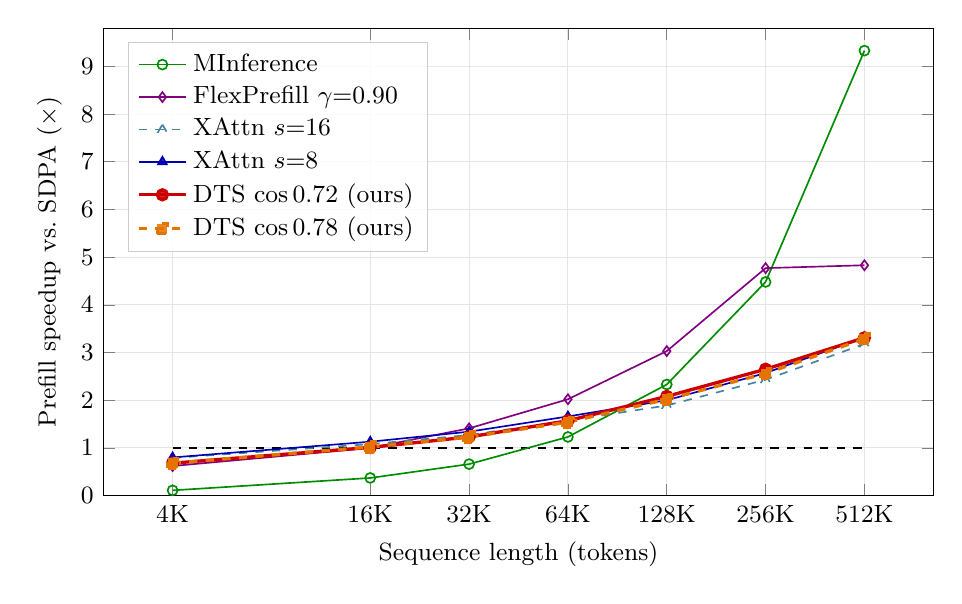
\begin{tikzpicture}
\begin{axis}[
    width=\linewidth, height=0.62\linewidth,
    xmode=log, log basis x=2,
    xtick={4096,16384,32768,65536,131072,262144,524288},
    xticklabels={4K,16K,32K,64K,128K,256K,512K},
    xlabel={Sequence length (tokens)},
    ylabel={Prefill speedup vs.\ SDPA ($\times$)},
    ymin=0, ymax=9.8,
    ytick={0,1,2,3,4,5,6,7,8,9},
    grid=both, grid style={gray!20},
    legend pos=north west,
    legend cell align=left,
    legend style={font=\small, fill=white, fill opacity=0.85, text opacity=1, draw=gray!40},
    tick label style={font=\small},
    label style={font=\small},
    mark size=1.8pt,
]
% break-even reference (SDPA)
\addplot[black, dashed, thick, forget plot] coordinates {(4096,1)(524288,1)};

\addplot[color=green!55!black, semithick, mark=o]
    coordinates {(4096,0.11)(16384,0.37)(32768,0.66)(65536,1.23)(131072,2.33)(262144,4.48)(524288,9.33)};
\addlegendentry{MInference}
\addplot[color=violet, semithick, mark=diamond]
    coordinates {(4096,0.62)(16384,1.00)(32768,1.41)(65536,2.02)(131072,3.03)(262144,4.77)(524288,4.83)};
\addlegendentry{FlexPrefill $\gamma{=}0.90$}
\addplot[color=cyan!60!black, semithick, dashed, mark=triangle]
    coordinates {(4096,0.79)(16384,1.08)(32768,1.27)(65536,1.57)(131072,1.89)(262144,2.43)(524288,3.18)};
\addlegendentry{XAttn $s{=}16$}
\addplot[color=blue!70!black, semithick, mark=triangle*]
    coordinates {(4096,0.80)(16384,1.13)(32768,1.34)(65536,1.66)(131072,2.00)(262144,2.57)(524288,3.32)};
\addlegendentry{XAttn $s{=}8$}
\addplot[color=red!80!black, very thick, mark=*]
    coordinates {(4096,0.68)(16384,1.01)(32768,1.23)(65536,1.57)(131072,2.08)(262144,2.65)(524288,3.31)};
\addlegendentry{DTS cos\,0.72 (ours)}
\addplot[color=orange!90!black, very thick, dashed, mark=square*]
    coordinates {(4096,0.68)(16384,1.02)(32768,1.23)(65536,1.54)(131072,2.02)(262144,2.56)(524288,3.29)};
\addlegendentry{DTS cos\,0.78 (ours)}
\end{axis}
\end{tikzpicture}
\caption{End-to-end prefill speedup relative to SDPA across sequence lengths on LLaMA-3.1 8B Instruct (4$\times$H100, layer-sharded). Points above the dashed break-even line (1.0$\times$) are faster than full attention.}
\label{fig:dts_speedup_trend}
\end{figure}

\subsection{Cosine threshold ablation}
\label{sec:results_cos_ablation}

The cosine threshold $\tau$ controls how aggressively DTS packs the delta representation used for tile scoring: a lower $\tau$ keeps fewer rows, making the score cheaper but less accurate, while a higher $\tau$ keeps more rows for a more accurate but more expensive score. We sweep $\tau \in \{0.70, 0.72, 0.75, 0.78, 0.80\}$ at fixed recall $r{=}0.90$ and report speedup, RULER, and LongBench. Because this sweep repeats the evaluation across five configurations, we use the reduced RULER (30 samples, 9 tasks) and reduced LongBench (9 tasks).

The sweep trades scoring cost against tile count, and the two roughly cancel out (Table~\ref{tab:cos_ablation}). Lower thresholds score faster (1.6\% of full tile cost, 1{,}447 ms at cos\,0.70) but need more tiles to reach 90\% attention mass, since the ranking is coarser (19.0\% of tiles, 3{,}094 ms of attention). Higher thresholds give a sharper ranking that hits the same recall with fewer tiles (13.3\% of tiles, 2{,}140 ms of attention at cos\,0.80) but cost more to score (8.7\%, 2{,}885 ms). Because scoring and attention move in opposite directions, the end-to-end speedup stays roughly flat: it peaks at cos\,0.72 (2.10$\times$), stays close at cos\,0.70 (2.08$\times$), and only drops off at the high end (2.03$\times$ at cos\,0.78, 1.97$\times$ at cos\,0.80).

RULER is essentially lossless across the whole sweep (Table~\ref{tab:cos_ablation}): every setting lands within 0.4 points of the others.

LongBench is more sensitive to $\tau$ (Table~\ref{tab:cos_ablation}). Accuracy peaks at cos\,0.72 (39.21) and falls off at both ends. cos\,0.72 is the best overall choice: fastest and best on LongBench. cos\,0.78 is the accuracy-maximizing choice, holding the best RULER score (91.80) at a still-good 2.03$\times$. We carry both forward as the two settings compared against the other methods.

\begin{table}[!ht]
\centering
\caption{End-to-end prefill speedup (128K tokens) and accuracy (\%) on RULER and LongBench for DTS cosine thresholds on LLaMA-3.1 8B Instruct. Attention density is the fraction of computed sparse attention. Score\% represents the scoring overhead. Score ms and Attn ms indicate the respective phase latencies.}
\label{tab:cos_ablation}
\resizebox{\linewidth}{!}{%
\begin{tabular}{lrrrrrrr}
\toprule
Method & Speedup & Density & Score\% & Score (ms) & Attn (ms) & RULER & LongBench \\
\midrule
Full attention & 1.00$\times$ & 100\% & -- & -- & -- & 91.52 & 39.54 \\
\midrule
cos\,0.70 & 2.08$\times$ & 19.0\% & 1.6\% & 1{,}447 & 3{,}094 & 91.69 & 38.95 \\
cos\,0.72 & 2.10$\times$ & 17.6\% & 2.3\% & 1{,}611 & 2{,}853 & 91.51 & 39.21 \\
cos\,0.75 & 2.09$\times$ & 15.7\% & 3.8\% & 1{,}954 & 2{,}545 & 91.42 & 39.08 \\
cos\,0.78 & 2.03$\times$ & 14.2\% & 6.3\% & 2{,}445 & 2{,}284 & 91.80 & 39.15 \\
cos\,0.80 & 1.97$\times$ & 13.3\% & 8.7\% & 2{,}885 & 2{,}140 & 91.58 & 38.61 \\
\bottomrule
\end{tabular}%
}
\end{table}
\subsection{Cross-Model Generalization: Qwen2.5-7B}
\label{sec:results_qwen}

The results above use LLaMA-3.1 8B Instruct throughout. To check whether DTS's behavior is specific to that model, we repeat the full RULER, LongBench, and speedup evaluation on Qwen2.5-7B-Instruct-1M, using the same two operating points (cos\,0.72 and cos\,0.78) and the same baselines.


\paragraph{RULER.}

Table~\ref{tab:delta_tile_scoring_qwen} reports RULER accuracy on Qwen. MInference (90.35) and both XAttention strides (90.25 at $s{=}16$, 90.23 at $s{=}8$) tie full attention (90.33); DTS trails by 1.4--2.2 points (88.89 at cos\,0.78 and 88.12 at cos\,0.72). FlexPrefill collapses to 53.50.

\begin{table}[!ht]
\centering
\caption{RULER accuracy (\%) comparing DTS with the other baselines on Qwen2.5-7B-Instruct-1M. Best score per column in \textbf{bold}. The DTS row is measured under the corrected scoring kernel; cos\,0.72 was not re-run under it and is omitted.}
\label{tab:delta_tile_scoring_qwen}
\resizebox{\linewidth}{!}{%
\begin{tabular}{lrrrrrrr}
\toprule
Method & 4K & 8K & 16K & 32K & 64K & 128K & Avg \\
\midrule
Full attention              & 94.10 & 93.67 & 93.54 & \textbf{91.17} & 88.07 & \textbf{81.41} & 90.33 \\
MInference                  & \textbf{94.16} & \textbf{94.00} & \textbf{94.03} & 90.99 & 87.68 & 81.23 & \textbf{90.35} \\
FlexPrefill                  & 74.39 & 61.74 & 55.66 & 59.71 & 32.38 & 37.10 & 53.50 \\
\midrule
XAttn $s{=}16$                & 94.02 & 93.55 & 93.66 & 90.85 & \textbf{88.21} & 81.22 & 90.25 \\
XAttn $s{=}8$                 & 94.06 & 93.53 & 93.60 & 91.02 & 87.96 & 81.23 & 90.23 \\
\midrule
DTS cos\,0.78 & 93.98 & 93.49 & 93.33 & 89.47 & 86.95 & 81.28 & 89.75 \\
\bottomrule
\end{tabular}%
}
\end{table}

To trace the source of this performance gap, we analyze the 13 individual RULER tasks at 128K. While DTS matches or beats XAttention on 11 tasks, it falls short on variable tracking (vt) and common word extraction (cwe). Both are aggregation tasks that require combining information from multiple positions rather than retrieving a single needle. DTS's performance drops sharply on these (e.g., 53.8 and 13.8 at cos\,0.72, compared to full attention's 75.8 and 27.3), indicating a trade-off where DTS remains strong on retrieval but struggles with broad aggregation.

\paragraph{LongBench.}

Table~\ref{tab:longbench_qwen} shows LongBench scores on Qwen. DTS ties full attention (46.76): 46.19 at cos\,0.72 and 46.20 at cos\,0.78, tracking both XAttention variants (46.46 at $s{=}8$, 46.66 at $s{=}16$).

DTS only underperforms full attention on MuSiQue (29.22--29.88 vs. 32.70) and 2WikiMultiHopQA (52.46--53.31 vs. 55.45). Because both are multi-hop tasks that require synthesizing evidence across passages, this result reinforces the aggregation limitation observed in RULER. Additionally, MInference's average is marked with a $\dagger$ because it failed to complete QMSum and RepoBench-P at 128K.

\begin{table*}[!ht]
\centering
\small
\caption{LongBench scores on Qwen2.5-7B-Instruct-1M. Task abbreviations as in Table~\ref{tab:longbench}. Best score per column in \textbf{bold}. As in Table~\ref{tab:delta_tile_scoring_qwen}, the DTS row is measured under the corrected scoring kernel; cos\,0.72 was not re-run under it and is omitted. $\dagger$MInference failed on 2 of 16 tasks (QMSum, RepoBench-P); no average is reported for it, since a mean over the 14 completed tasks omits two below-average tasks and is not comparable to the other rows.}
\label{tab:longbench_qwen}
\resizebox{\linewidth}{!}{%
\begin{tabular}{lrrrrrrrrrrrrrrrrr}
\toprule
Method & NQA & Qas & MFQ & HotP & 2Wiki & Mus & GovR & QMS & MNews & TREC & TQA & SAM & PCnt & PassR & LCC & RepoB & Avg \\
\midrule
Full attention               & 29.26 & 45.12 & 51.49 & \textbf{58.34} & 55.45 & 32.70 & 35.22 & 23.99 & 25.69 & 71.00 & 83.31 & 45.24 & 10.00 & \textbf{100.00} & 48.40 & 32.92 & 46.76 \\
MInference$^\dagger$         & 29.38 & 45.36 & 51.85 & 56.77 & 54.65 & \textbf{33.47} & 35.20 & --    & 25.98 & 71.00 & 83.31 & \textbf{46.32} & 10.00 & 99.00 & 47.63 & --    & --    \\
FlexPrefill                  & 24.68 & 39.46 & 50.63 & 48.72 & 50.58 & 21.06 & 33.61 & \textbf{24.67} & 25.42 & 70.00 & 78.64 & 46.11 & 2.00 & 59.00 & 45.18 & 33.61 & 40.84 \\
XAttn $s{=}16$               & 29.84 & 44.74 & 51.41 & 57.63 & \textbf{55.62} & 32.60 & 34.84 & 24.00 & \textbf{26.09} & 70.00 & 83.18 & 46.00 & \textbf{12.00} & \textbf{100.00} & 46.70 & 31.97 & 46.66 \\
XAttn $s{=}8$                & \textbf{30.26} & \textbf{45.77} & 52.31 & 58.16 & 53.78 & 31.62 & 35.18 & 24.09 & 26.00 & 71.00 & 83.51 & 45.83 & 9.00 & \textbf{100.00} & 45.14 & 31.70 & 46.46 \\
\midrule
DTS cos\,0.78 & 21.96 & 44.66 & \textbf{53.08} & 54.57 & 54.63 & 33.21 & \textbf{35.47} & 24.12 & 25.64 & \textbf{74.00} & \textbf{84.19} & 46.13 & 6.00 & \textbf{100.00} & \textbf{48.49} & \textbf{33.71} & 46.24 \\
\bottomrule
\end{tabular}%
}
\end{table*}

\paragraph{Speedup.}

Figure~\ref{fig:dts_speedup_trend_qwen} illustrates end-to-end speedups on Qwen up to 512K (DTS and XAttention are capped at 256K due to OOM errors). The trends largely reflect those seen on LLaMA. MInference is the slowest up to 64K but overtakes FlexPrefill at 512K, reaching 4.81$\times$ (a smaller gain than on LLaMA). FlexPrefill is the fastest up to 256K before dipping to 3.87$\times$ at 512K. DTS and XAttention perform similarly, though DTS maintains a clear speed advantage at 128K and 256K (1.57$\times$ and 1.81$\times$ vs. XAttention's 1.45$\times$ and 1.74$\times$).

\begin{figure}[!ht]
\centering
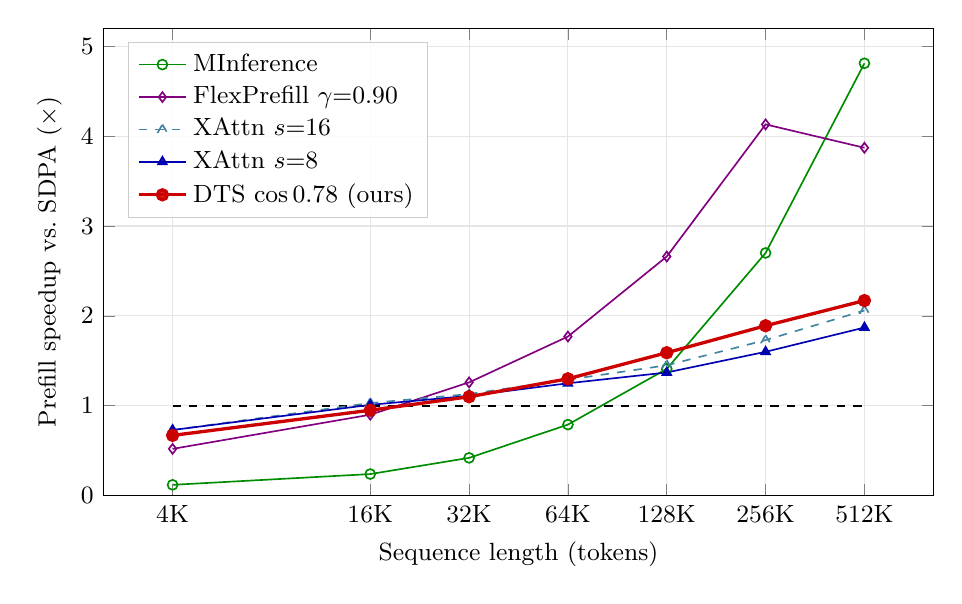
\begin{tikzpicture}
\begin{axis}[
    width=\linewidth, height=0.62\linewidth,
    xmode=log, log basis x=2,
    xtick={4096,16384,32768,65536,131072,262144,524288},
    xticklabels={4K,16K,32K,64K,128K,256K,512K},
    xlabel={Sequence length (tokens)},
    ylabel={Prefill speedup vs.\ SDPA ($\times$)},
    ymin=0, ymax=5.2,
    ytick={0,1,2,3,4,5},
    grid=both, grid style={gray!20},
    legend pos=north west,
    legend cell align=left,
    legend style={font=\small, fill=white, fill opacity=0.85, text opacity=1, draw=gray!40},
    tick label style={font=\small},
    label style={font=\small},
    mark size=1.8pt,
]
% break-even reference (SDPA)
\addplot[black, dashed, thick, forget plot] coordinates {(4096,1)(524288,1)};

\addplot[color=green!55!black, semithick, mark=o]
    coordinates {(4096,0.12)(16384,0.24)(32768,0.42)(65536,0.79)(131072,1.41)(262144,2.70)(524288,4.81)};
\addlegendentry{MInference}
\addplot[color=violet, semithick, mark=diamond]
    coordinates {(4096,0.52)(16384,0.90)(32768,1.26)(65536,1.77)(131072,2.66)(262144,4.13)(524288,3.87)};
\addlegendentry{FlexPrefill $\gamma{=}0.90$}
\addplot[color=cyan!60!black, semithick, dashed, mark=triangle]
    coordinates {(4096,0.73)(16384,1.03)(32768,1.13)(65536,1.29)(131072,1.45)(262144,1.73)(524288,2.06)};
\addlegendentry{XAttn $s{=}16$}
\addplot[color=blue!70!black, semithick, mark=triangle*]
    coordinates {(4096,0.73)(16384,1.01)(32768,1.11)(65536,1.25)(131072,1.37)(262144,1.60)(524288,1.87)};
\addlegendentry{XAttn $s{=}8$}
\addplot[color=red!80!black, very thick, mark=*]
    coordinates {(4096,0.67)(16384,0.95)(32768,1.10)(65536,1.30)(131072,1.59)(262144,1.89)(524288,2.17)};
\addlegendentry{DTS cos\,0.78 (ours)}
\end{axis}
\end{tikzpicture}
\caption{End-to-end prefill speedup relative to SDPA across sequence lengths on Qwen2.5-7B-Instruct-1M (4$\times$H100, layer-sharded). Points above the dashed break-even line (1.0$\times$) are faster than full attention.}
\label{fig:dts_speedup_trend_qwen}
\end{figure}

\subsection{Video Understanding: Qwen2-VL}
\label{sec:results_video}

We evaluate DTS on Video-MME (1 fps, no subtitles) using Qwen2-VL-7B-Instruct. We empirically observed that packing by Euclidean distance yields better performance on video tokens than cosine similarity, so we report DTS using Euclidean packing (see Appendix~\ref{app:videomme_ablations} for this ablation study). We measure accuracy on the full test set (2,700 videos) and prefill speedup (attention latency only) on a 10-video timing sample per duration split. 

Table~\ref{tab:videomme_main} reports results against the same baselines used in text experiments. DTS at $\delta{=}15$ is our primary configuration. It closely tracks full attention accuracy (60.8 vs. 62.1 overall) while providing the best balance of speed and accuracy on the critical long-video split: it scores 52.6 and runs at 1.33$\times$ full attention, outperforming XAttention (51.7, 1.18$\times$). MInference retains the highest accuracy (62.4) but remains slower than full attention across all buckets. FlexPrefill provides the highest speedup (2.18$\times$) but trails DTS in long-video accuracy (51.6).

\begin{table}[!ht]
\centering
\caption{Video-MME accuracy and prefill speedup on Qwen2-VL-7B-Instruct (Video-MME @ 1fps, no subtitles). Accuracy (\%) is on the full test set ($n{=}2700$). Speedup ($\times$full) is attention-kernel latency (self\_attn\_ms) relative to full attention on a 10-videos-per-bucket timing sample. Best accuracy per column in \textbf{bold}.}
\label{tab:videomme_main}
\resizebox{\linewidth}{!}{%
\begin{tabular}{lrrrrrrr}
\toprule
 & \multicolumn{4}{c}{Accuracy (\%)} & \multicolumn{3}{c}{Speedup ($\times$full)} \\
\cmidrule(lr){2-5}\cmidrule(lr){6-8}
Method & Short & Med & Long & Avg & Short & Med & Long \\
\midrule
Full attention                    & 72.3 & 61.0 & 53.0 & 62.1 & 1.00 & 1.00 & 1.00 \\
MInference                        & \textbf{72.8} & 61.2 & \textbf{53.3} & \textbf{62.4} & 0.42 & 0.62 & 0.61 \\
FlexPrefill                        & 72.1 & \textbf{61.3} & 51.6 & 61.7 & 1.41 & 2.12 & 2.18 \\
XAttn $s{=}16$                    & 72.0 & 59.9 & 51.7 & 61.2 & 0.95 & 1.22 & 1.18 \\
\midrule
DTS $\delta{=}15$                 & 71.1 & 58.6 & 52.6 & 60.8 & 0.98 & 1.21 & 1.33 \\
\bottomrule
\end{tabular}%
}
\end{table}

